%%%%%%%%%%%%%%%%%%%%%%%%%%%%%%%%%%%%%%%%%%%%%%%%%%%%
%%%% En-tête leçon
\begin{headerBlock}
  \chapter{Diffraction sur des structures périodiques}
    \label{LP_DiffractionPeriodique}
\end{headerBlock}

%%%%%%%%%%%%%%%%%%%%%%%%%%%%%%%%%%%%%%%%%%%%%%%%%%%%
%%%% Références
\begin{center}
\begin{tabularx}{\textwidth}{| X | X | c | c |}
  \hline
  \rowcolor{gray!20}\multicolumn{4}{c}{Bibliographie de la leçon : } \\
  \hline 
  Titre & Auteurs & Editeur (année) & ISBN \\
  \hline
   Physique du solide & Ashcroft et Mermin & EDP Sciences &   \\
  \hline 
   Tout-en-un MP & M.-N. Sanz & Dunod (2009) &  \\
  \hline 
  Optique & J.-P. Pérez & Dunod & \\
  \hline 
  Optique Physique et électronique & D. Mauras & PUF (2011à) & \\
  \hline
\end{tabularx}
\end{center}



%%%%%%%%%%%%%%%%%%%%%%%%%%%%%%%%%%%%%%%%%%%%%%%%%%%%
\begin{reportBlock}{Plan détaillé}
  \textbf{Niveau choisi pour la leçon :} Licence
  \newline
  \textbf{Prérequis : }Diffraction de Fraunhofer, trigonométrie, interférences, fente d'Young, théorème de Malus
  \newline
  
  \textbf{Déroulé détaillé de la leçon: }   \newline
On a pu voir des phénomènes de diffraction (ex : tâche d'airy). Cependant le papillon machin a des ailes bleues, la couleur disparaît lorsqu'on ajoute de l'eau.
  \section{Diffraction à deux pupilles}
  \subsection{Translation d'une pupille}
  \begin{center}
      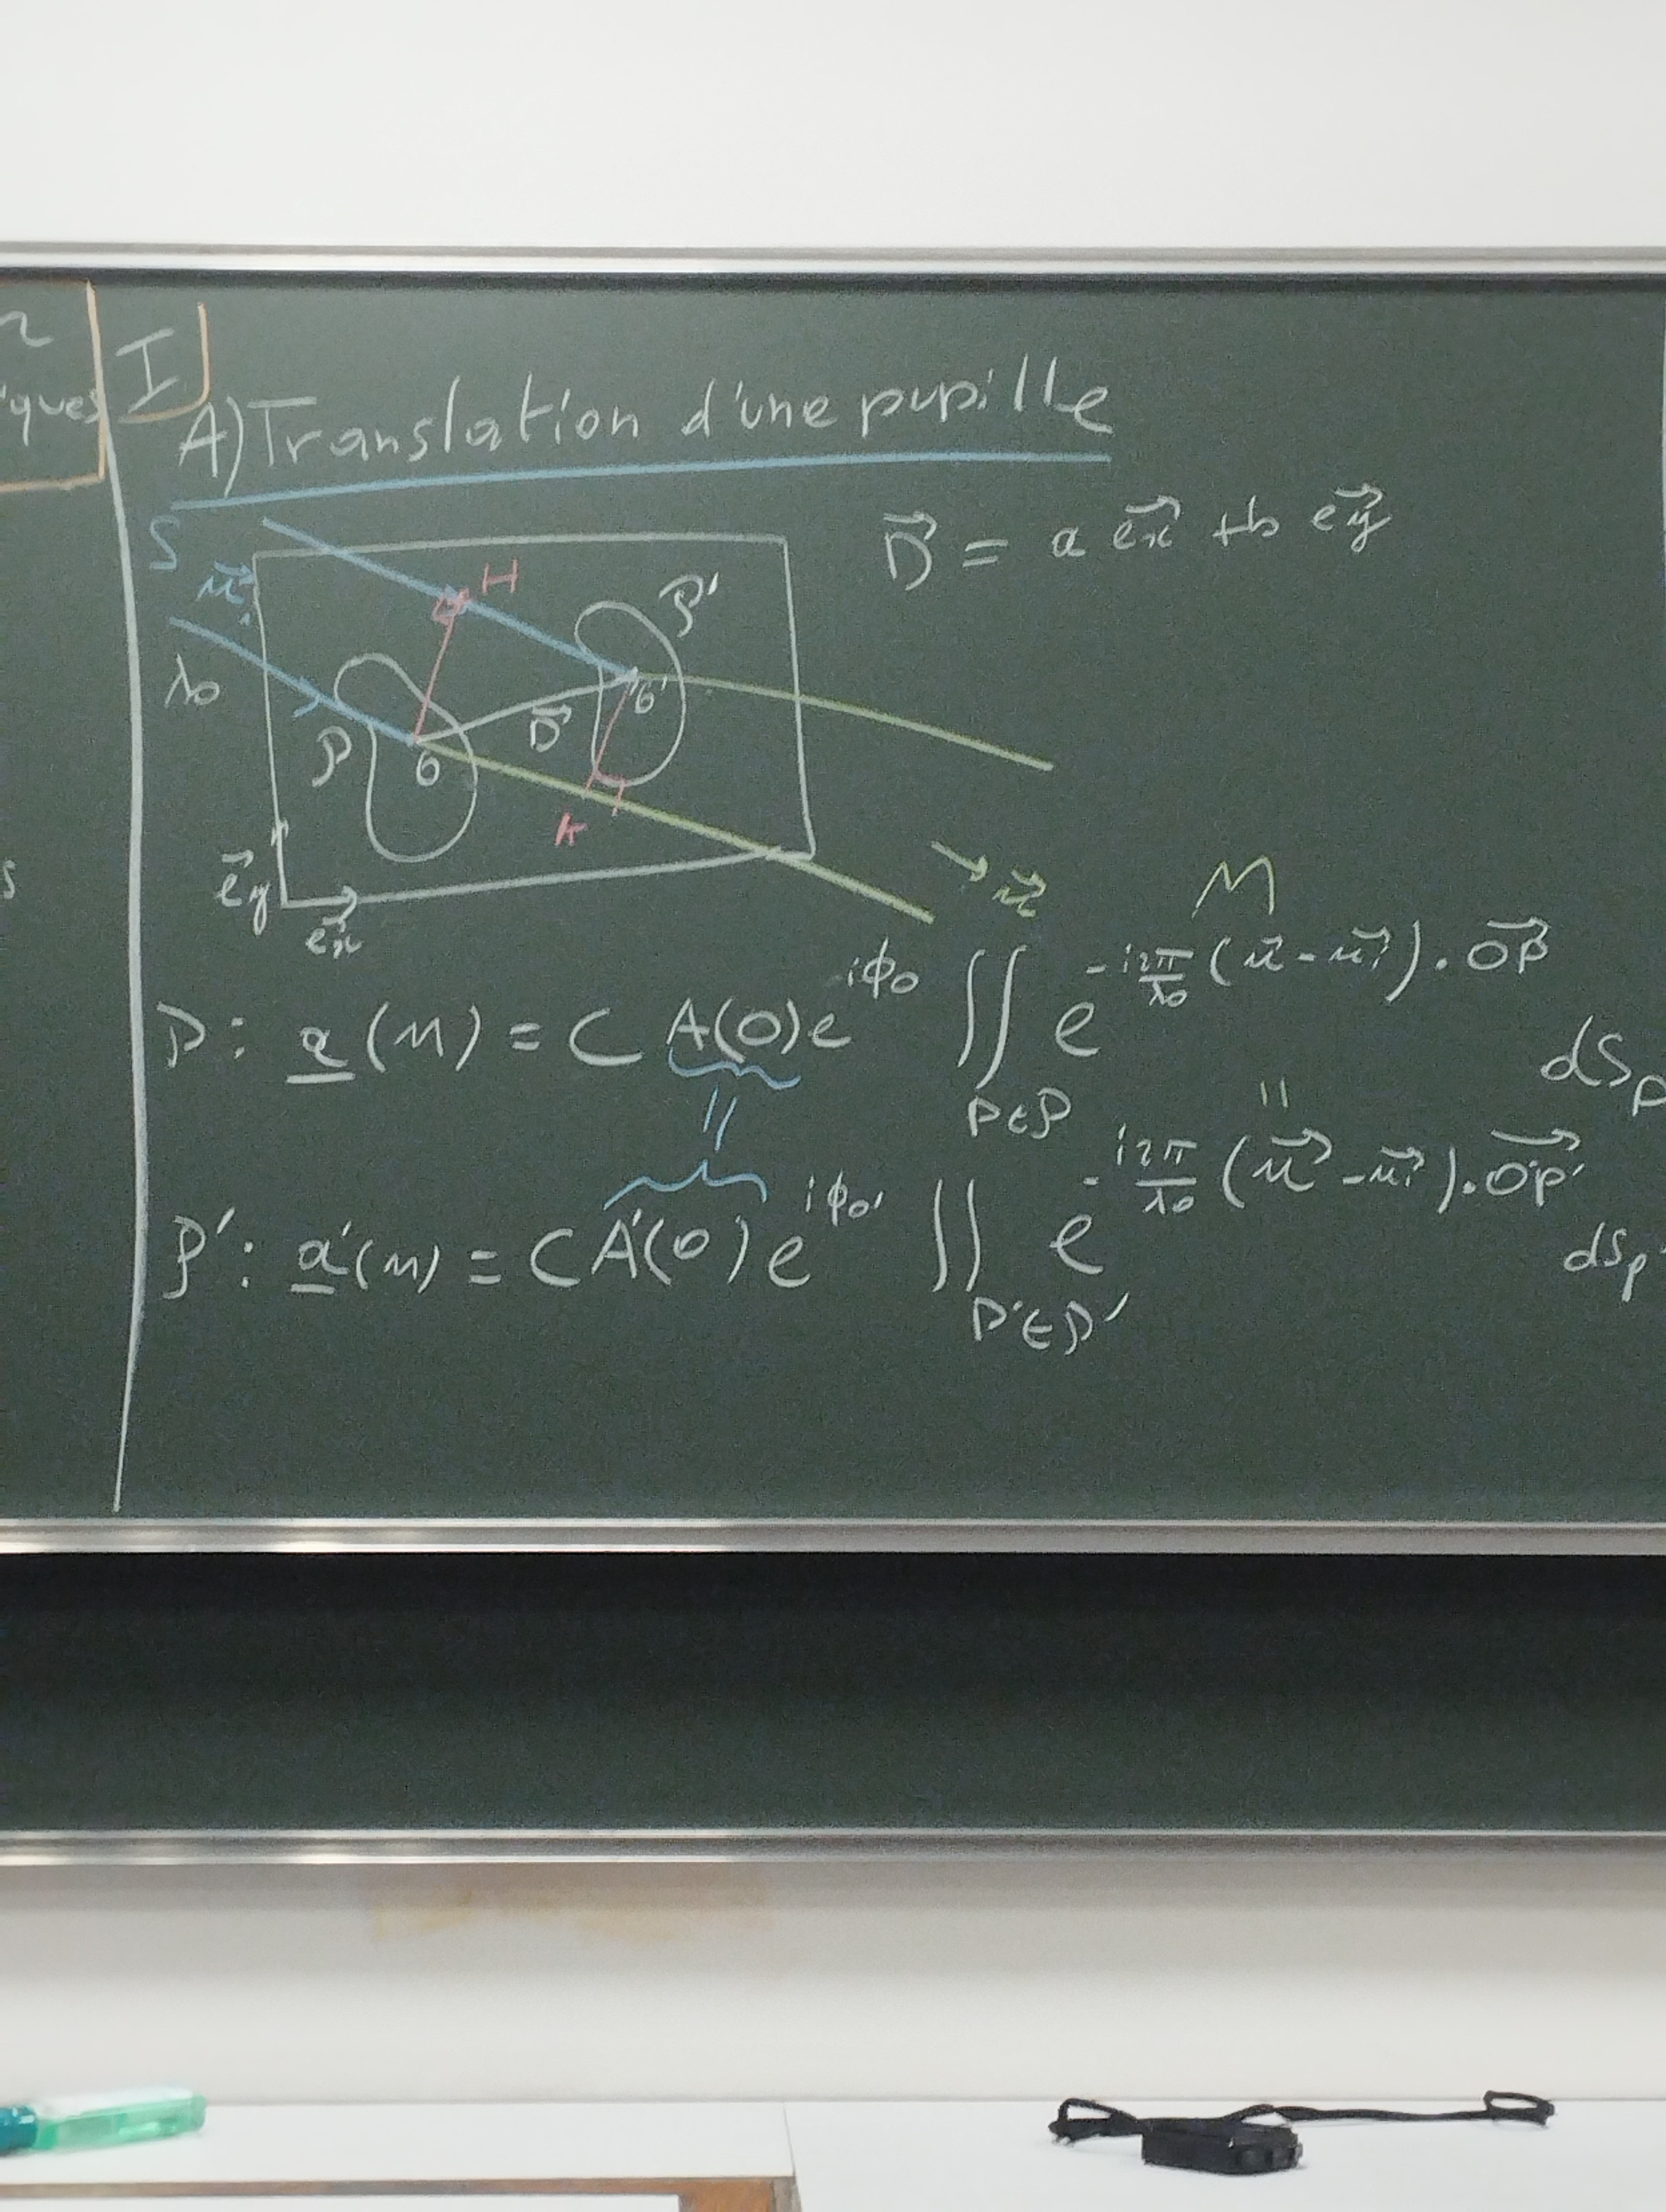
\includegraphics[scale=0.1]{LP_DiffractionPeriodique/Translation_pupille.jpg}
  \end{center}
  En utilisant la diffraction de Fraunhofer :
  \begin{itemize}
      \item \underline{a}(M)$=CA(O)\exp{j\phi_0} \int_{p\in P} \exp{j\frac{2\pi}{\lambda_0}(\mathbf{u}-\mathbf{u_i})\cdot \mathbf{OP}} \, \mathrm{dS_p} $
      \item \underline{a}(M)$=CA^{'}(O)\exp{j\phi_0} \int_{p\in P^{'}} \exp{j\frac{2\pi}{\lambda_0}(\mathbf{u}-\mathbf{u_i})\cdot \mathbf{OP^{'}}} \, \mathrm{dS_p^{'}} $
  \end{itemize}
  On en déduit le déphasage $\Delta \phi = \frac{2\pi}{\lambda_0}(\mathbf{u}-\mathbf{u_i})\cdot\mathbf{D}$. Comme l'éclairement $\epsilon\propto$\underline{a}\underline{a$^{'*}$} est proportionnel, cela va avoir des conséquences.

  \subsection{Diffraction de deux fentes d'Young}
  \textcolor{red}{Attention, erreur dans la formule (cf question)}.
  \begin{equation}
      \epsilon = a_1 a_1^* + 2(1+cos(\Delta\phi))
  \end{equation}
  Le premier terme vient de la diffraction, le second est un terme d'interférences.

  \section{Diffraction sur un réseau}
  \subsection{Caractéristiques}
  On note $a$ le pas du réseau.
  \subsection{Loi des réseaux}
  \begin{center}
      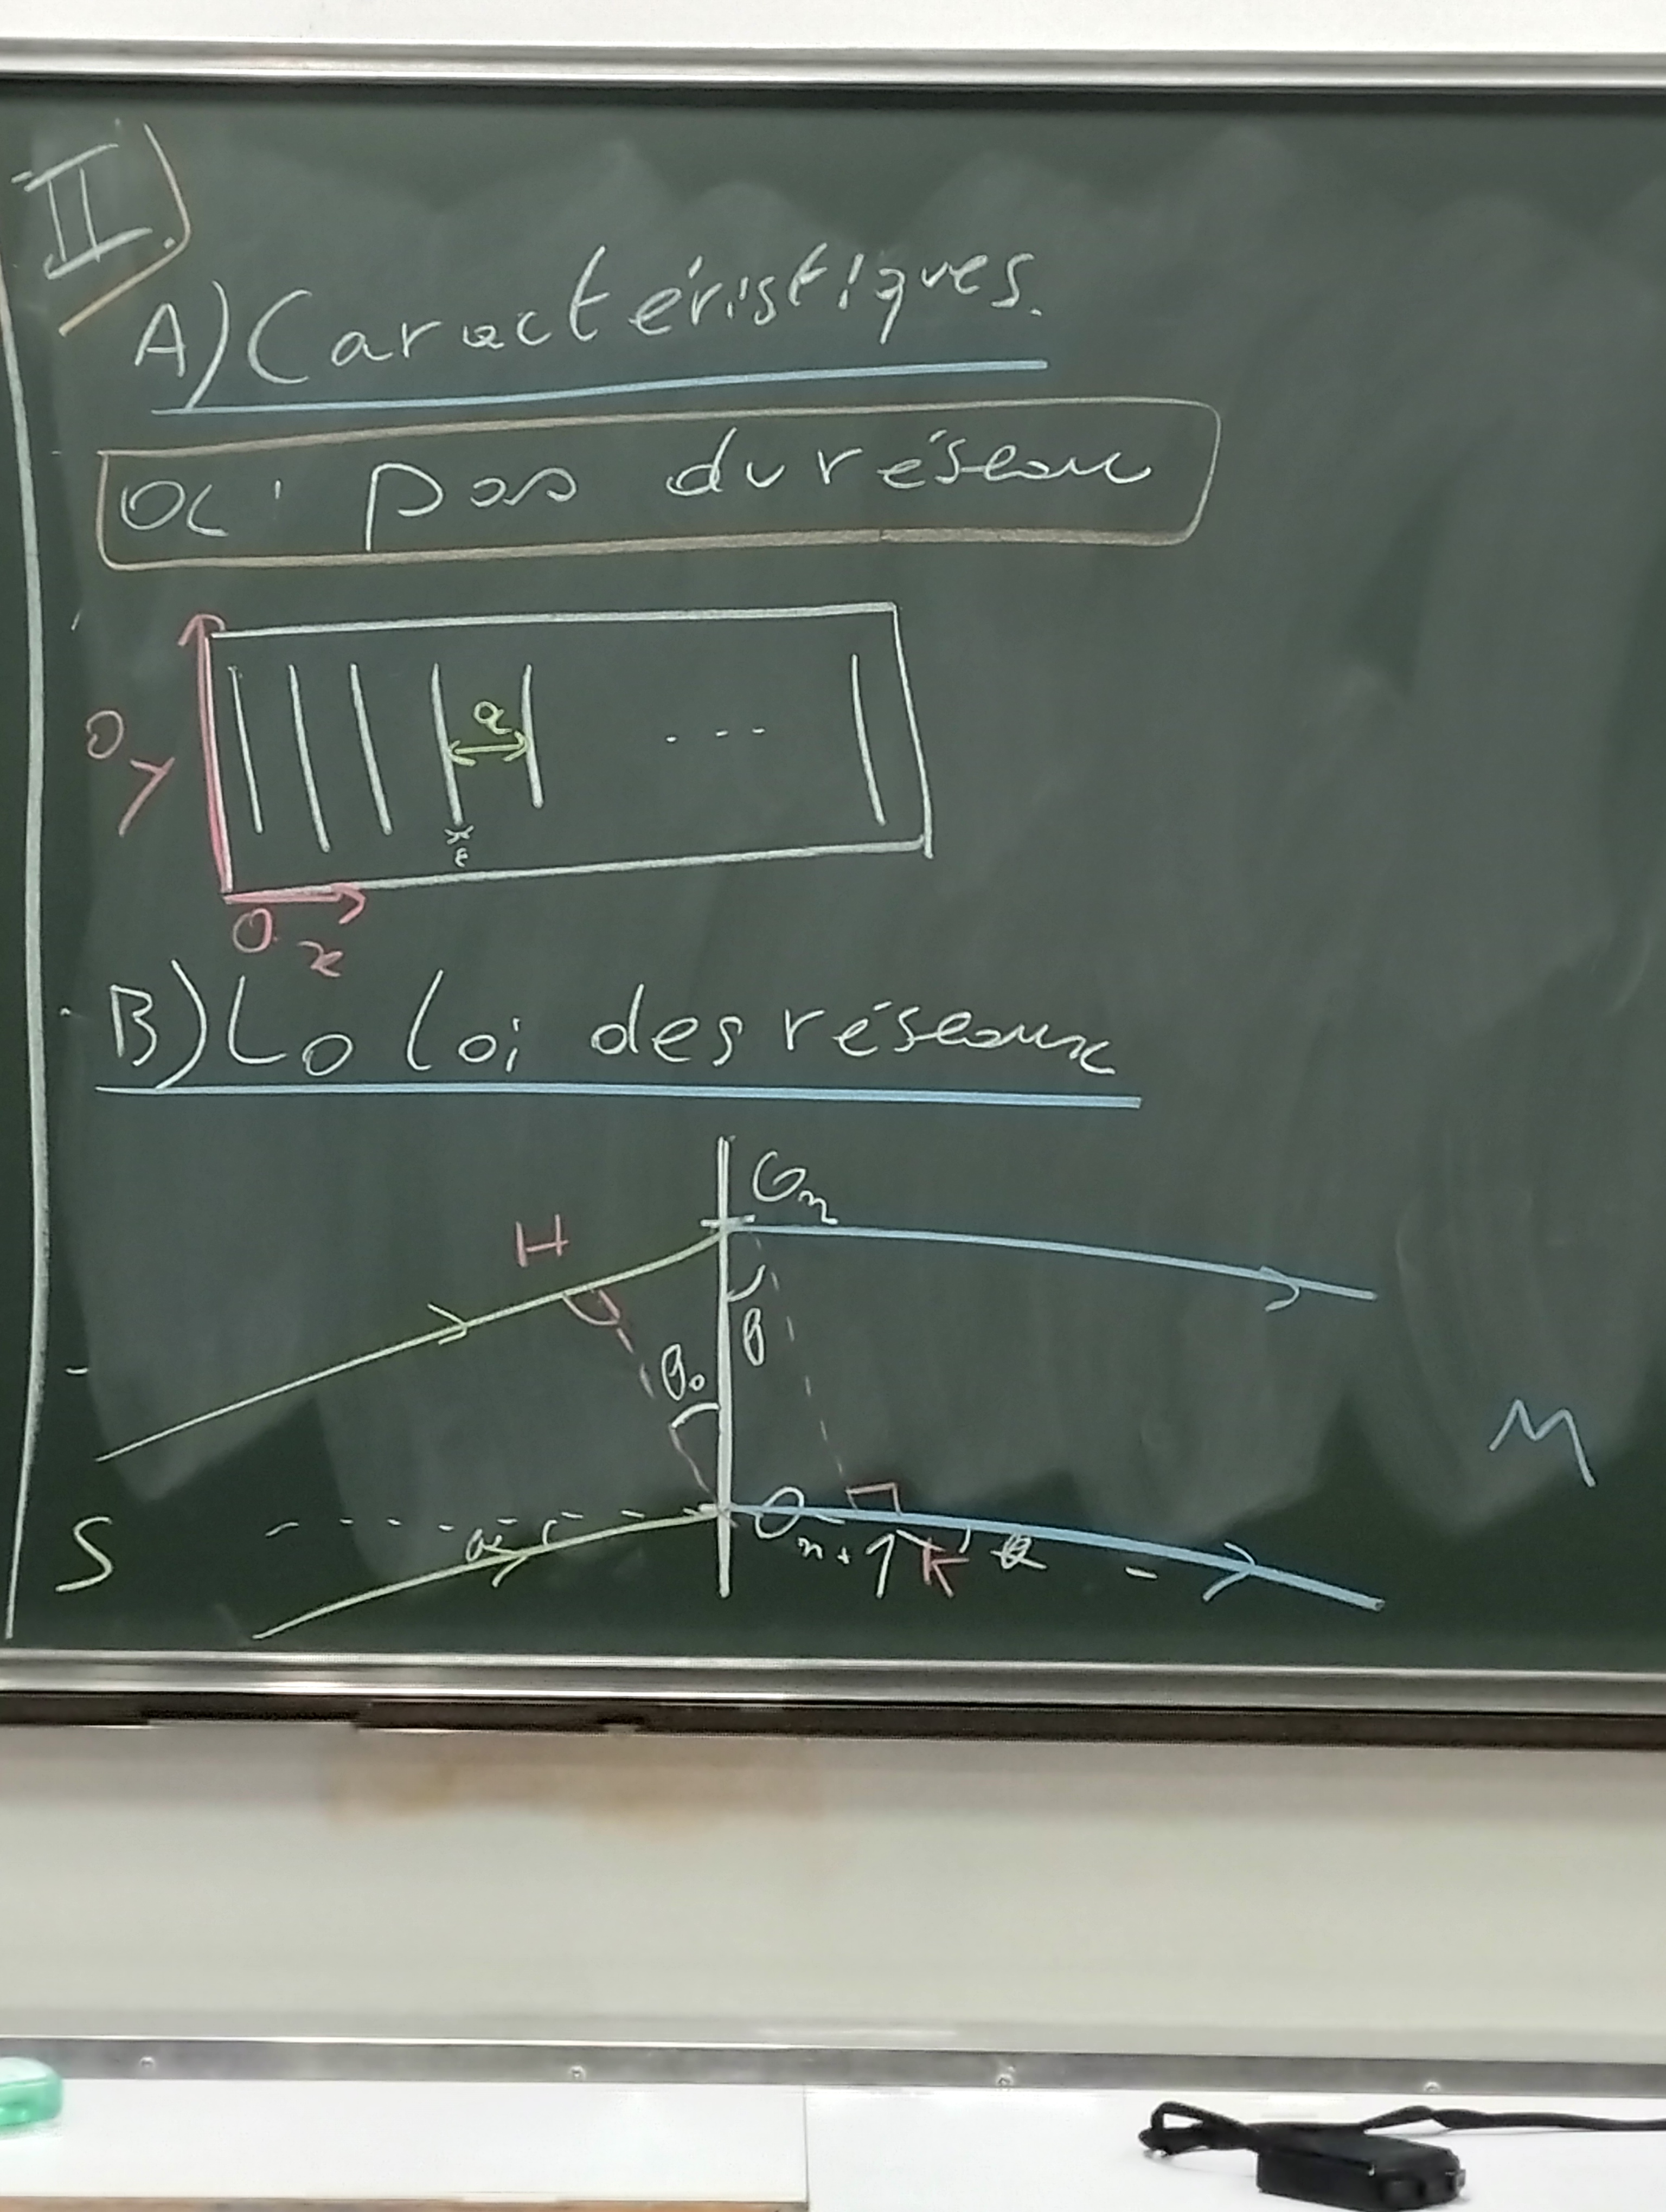
\includegraphics[scale=0.1]{LP_DiffractionPeriodique/Reseau.jpg}
  \end{center}
  La différence de marche vaut :
\begin{align*}
\delta &= O_{n+1}M-O_{n}M \\
           &= a\sin{\theta} - a\sin{\theta_0}
\end{align*}
La formule des réseaux est donc :
\begin{equation}
    n\frac{\lambda}{a} = \sin{\theta_n} - a\sin{\theta_0}
\end{equation}
avec $n$ l'ordre de l'interférence.

\subsection{Diffraction d'une source ponctuelle}
Mise en application : \textcolor{green}{Montage de la mise en évidence de le diffraction d'un faisceau laser sur un réseau.} Mesure du pas du réseau par la mesure de l'écartement des tâches de diffraction et de la distance réseau-écran. 

\section{Conclusion}
Ouverture sur la diffraction des rayons X. Tâches de diffraction des papillons.
\end{reportBlock}


\begin{reportBlock}{Questions posées par l’enseignant (avec réponses)}
  \textbf{C : Quelles sont les conditions d'observation de la manip ?}  \textcolor{purple}{Fraunhofer (image et objet à l'infini)}. Une source ponctuelle ça envoie des rayons parallèles à l'infini ? \textcolor{purple}{Dans le cas du laser, oui (presque à l'infini).} Dessine moi le montage de Fraunhofer. Est-on dans les conditions de Fraunhofer ? \textcolor{purple}{Non il manque une lentille à la sortie du réseau.}\\
  \textbf{C : Choix du papier millimétré ?}  \textcolor{purple}{Cela me servait d'aide pour les mesures.}\\
   \textbf{C : Si on avait utilisé une caméra CCD, qu'aurait-on obtenu ?}  \textcolor{purple}{On aurait obtenu un sinus cardinal en enveloppe avec un phénomène d'interférence à l'intérieur.} Comment influe une variation des paramètres sur cette figure ? \textcolor{purple}{L'espacement entre les maxima est inversement proportionnel au pas du réseau. La largeur à mi-hauteur du sinus cardinal est } \\
   \textbf{C : Revenons à la formule de l'éclairement à travers deux fentes d'Young.}  \textcolor{purple}{Ce n'est pas une somme, c'est un produit...} C'est quoi le nom des deux termes ? \textcolor{purple}{Facteur de forme (le premier) et facteur de structure (le second)}\\
   \textbf{C : C'est quoi l'éclairement $\epsilon$ ? Lien entre éclairement et intensité $I$ ?}  \textcolor{purple}{On a $\epsilon = KI = K<s^2(M,t)>$, où $<...>$ représente la valeur moyenne temporelle, K est une constante qui dépend du détecteur et $s(M,t)$ représente une composante du champ électrique de la lumière par rapport à un axe perpendiculaire à sa direction de propagation. L'éclairement est la puissance surfacique moyenne de l'onde lumineuse (autrement dit la valeur moyenne du vecteur de Poynting).}
   \textbf{C : A quoi ça sert les rayons X ?}  \textcolor{purple}{A sonder la matière.} Où sont les pupilles qui diffractent dans la matière ? \textcolor{purple}{Atomes = n\oe uds du réseau. Distance entre les plans d'atomes = pas du réseau}
\end{reportBlock}

%%%%%%%%%%%%%%%%%%%%%%%%%%%%%%%%%%%%%%%%%%%%%%%%%%%%
%%%% Correction
\begin{reportBlock}{Partie réservée au correcteur}
  \textbf{Avis général sur la leçon (plan, contenu, etc.)}
  
  
  \textbf{Notions fondamentales à aborder, secondaires, délicates :}
  
  
  
  \textbf{Expériences possibles (en particulier pour l'agrégation docteur) :}
  
  
  \textbf{Bibliographie conseillée : }

\end{reportBlock}